% Plantilla, paquetes, macros, etc. para los proyectos en latex realizados por Eduardo Gavazut, Universidad Simón Bolívar
% Este .tex se deriva directamente del utilizado de las notas, así que probablemente hayan muchos paquetes y macros sin utilizar

\documentclass{article}
\usepackage[utf8]{inputenc}
\usepackage{parskip}
\usepackage{amssymb, amsthm, amsmath, fdsymbol, mathtools} % Varios paquetes para símbolos y fuentes
\usepackage{tikz, pgfplots} % Para dibujar
\usepackage{tkz-graph, tkz-berge} % Para dibujar grafos
\usepackage[linguistics]{forest} % Para dibujar árboles
\usepackage{titling} % Para estilizar el título
\usepackage{scrextend} % Añade márgenes para hacer bloques de texto
\usepackage{enumitem} % Para enumerar sin sangría
\usepackage{graphicx, subcaption, wrapfig} % Para colocar figuras e imágenes
\usepackage{lastpage}
\usepackage{fancyhdr} % Para hacer encabezados y pie de página más estilizados
\usepackage{color} % Para usar colores en el texto
\usepackage{soul} % Para subrayar con colores
\usepackage{geometry}
\usepackage{hyperref}
\usepackage{booktabs} % Para hacer tablas un poco más estilizadas
\usepackage{multirow}

% Cambia el tamaño de los captions
\usepackage[font={footnotesize}]{caption}

% Establece los enviroments para teoremas, ejemplos, definiciones, etc

\newtheorem{teo}{Teorema}
\newtheorem{cor}[teo]{Corolario}
\newtheorem{lem}[teo]{Lema}
\newtheorem{pro}[teo]{Proposición}
\newtheorem{pre}{Pregunta}

\theoremstyle{definition}
\newtheorem{defn}{Definición}
\newtheorem{ejem}{Ejemplo}
\newtheorem{ejer}{Ejercicio}
\newtheorem{notn}{Notación}
\newtheorem{nota}{Nota}
\newtheorem{prob}{Problema}

% Comandos para símbolos
\newcommand{\R}{\mathbb{R}}
\newcommand{\Z}{\mathbb{Z}}
\newcommand{\N}{\mathbb{N}}

% Cambia el nombre de varios comandos
\renewcommand{\contentsname}{Contenido}
\renewcommand*{\proofname}{Demostración}
\renewcommand{\figurename}{Fig.}

% Cambia los márgenes
\geometry{
    left=20mm,
    right=20mm,
}

% Resetea el contador de ecuaciones en cada sección
\newcounter{sec}
\setcounter{sec}{0}
\counterwithin*{equation}{sec}
\counterwithin*{ejer}{sec}

% Establecemos cómo será el encabezado y el pie de página
\fancyhf{}
\pagestyle{fancy}
\fancyhf{}
\fancyhead[L]{MA3712}
\fancyhead[C]{Eduardo José Gavazut Pinto}
\fancyhead[R]{13-10524}
\fancyfoot[L]{Sección 1}
\fancyfoot[R]{Profesor: Daniel Morales}
\fancyfoot[C]{\thepage\ de \pageref{LastPage}}
\renewcommand{\headrulewidth}{2pt} 
\renewcommand{\footrulewidth}{2pt}

% Añade color a los lados de los grafos tikz
\tikzset{
    EdgeStyle/.append style = {blue}
}

% Permite agregar etiquetas a los niveles de un árbol
\forestset{%
  label tree/.style={
    for tree={tier/.option=level},
    level label/.style={
      before typesetting nodes={
        for nodewalk={current,tempcounta/.option=level,group={root,tree breadth-first},ancestors}{if={>OR={level}{tempcounta}}{before drawing tree={label me=##1}}{}},
      }
    },
    before drawing tree={
      tikz+={\coordinate (a) at (current bounding box.east);},
    },
  },
  label me/.style={tikz+={\node [anchor=base north] at (.parent |- a) {#1};}},
}

% Establece el subrayado de color rojo
\definecolor{ferrari}{rgb}{1,0.17,0}
\setulcolor{ferrari}

% Reduce el espacio entre el título y el header
\setlength{\droptitle}{-5.5em}
\renewcommand\maketitlehookc{\vspace{-3ex}}

% Define el espaciado entre párrafos
\setlength{\parskip}{1.5em}

% Definimos nuestro título
\pretitle{\begin{flushleft}\LARGE\sffamily}
\title{
Ecuaciones Diferenciales 1\\
Universidad Simón Bolívar
}
\posttitle{\par\end{flushleft}\vskip 0.5em}
\preauthor{\begin{flushleft}\large\scshape}
\author{
Eduardo Gavazut \\
Carnet: 13-10524}
\postauthor{\par\end{flushleft}}
\predate{\begin{flushleft}\large\scshape}
\date{Enero - Marzo 2024}
\postdate{\par\end{flushleft}}

% Aquí empieza el documento
\pgfplotsset{compat=1.18}
\begin{document}

\maketitle
\thispagestyle{fancy}

\section{Repaso de Derivada}
\stepcounter{sec}

Haremos primero un repaso de la derivada, concepto fundamental del cálculo diferencial. Trataremos ante todo las derivadas de funciones de una variable real, más especialmente de funciones reales definidas en intervalos de $\R$.

\begin{defn}
    Sea $f$ una función real definida en un intervalo abierto $(a, b)$, y supongamos que $c \in \R$ es un punto tal que $c \in (a, b)$. Diremos que $f$ es diferenciable en $c$ siempre que el límite
    
    \[
    \lim_{x \to c} \frac{f(x) - f(c)}{x-c}
    \]
    
    \noindent exista. Este límite, denotado por $f'(c)$ se llama \ul{derivada} de $f$ en $c$.
\end{defn}

Esta forma de calcular límites define una nueva función $f'$ cuyo dominio está formado por aquellos puntos de $(a, b)$ en los que $f$ es diferenciable. La función $f'$ se llama la \ul{primera derivada} de $f$. De forma análoga, la $n$-ésima derivada de $f$ se designa por $f^{(n)}$, y es la primera derivada de $f^{(n-1)}$, para $n = 2, 3, \dots$

\begin{teo}[Teorema del Valor Medio (T.V.M)]\label{teo:1.1.1}
    Si $f$ está definida en un intervalo $(a, b)$ y es diferenciable en un punto $c$ de $(a, b)$, entonces existe una función $f^*$ (que depende de $f$ y $c$) continua en $c$ y que satisface la ecuación
    
    \begin{equation}\label{eq:1.1.1}
        f(x) - f(c) = (x-c)f^*(x)
    \end{equation}
    
    \noindent para todo $x$ de $(a, b)$, con $f^*(c) = f'(c)$. Recíprocamente, si existe una función $f^*$ continua en $c$, que satisface la ecuación anterior, entonces $f$ es diferenciable en $c$ y $f'(c) = f^*(c)$.
\end{teo}

\begin{proof}
    Si $f$ es diferenciable en $c$, entonces $f'(c)$ existe. Definamos ahora $f^*$  en $(a, b)$ como sigue:
    
    \[
    f^*(x) = 
    \begin{cases}
        \dfrac{f(x) - f(c)}{x-c} & \text{si $x \neq c$} \\
        f'(c) & \text{e.o.c}
    \end{cases}
    \]
    
    Entonces $f^*$ es continua en $c$ y \ref{eq:1.1.1} se verifica para todo $x$ de $(a, b)$.
    
    Recíprocamente, si \ref{eq:1.1.1} se verifica para alguna función $f^*$ continua en $c$, entonces dividiento por $x-c$ y haciendo tender $x$ a $c$, vemos que $f'(c)$ existe y es igual a $f^*(c)$.
\end{proof}

Como consecuencia directa de este teorema tenemos:

\begin{teo}
    Si $f$ es diferenciable en $c$, entonces $f$ es continua en $c$.
\end{teo}

\begin{proof}
    Se demostró en el teorema anterior. Basta con hacer $x \to c$.
\end{proof}

Ahora describiremos las fórmulas para diferenciar la suma, la resta, el producto, y el cociente de dos funciones:

\begin{teo}
    Supongamos que $f$ y $g$ están definidas en $(a, b)$ y son diferenciables en $c$. Entonces $f+g$, $f-g$ y $f \cdot g$ son también diferenciables en $c$. Esto es así para $f / g$ si $g(c) \neq 0$. Las derivadas de $c$ están dadas por
    
    \begin{enumerate}
        \item $(f \pm g)'(c) = f'(c) \pm g'(c)$.
        \item $(f \cdot g)'(c) = f(c)g'(c) + f'(c)g(c)$.
        \item $(f/g)'(c) = \dfrac{g(c)f'(c) - f(c)g'(c)}{g(c)^2}$, si $g(c) \neq 0$.
    \end{enumerate}
\end{teo}

Y finalmente, describiremos la regla de la cadena:

\begin{teo}[Regla de la cadena]
    Sea $f$ definida en un intervalo abierto $S$ y sea $g$ definida en $f(S)$ y consideremos la función compuesta $g \circ f$ definida en $S$ por medio de la ecuación
    
    \[
    (g \circ f)(x) = g(f(x))
    \]
    
    Supongamos que existe un punto $c$ de $S$ tal que $f(c)$ sea un punto interior de $f(S)$. Si $f$ es diferenciable en $c$ y $g$ es diferenciable en $f(c)$, entonces $g \circ f$ es diferenciable en $c$ y se tiene que
    
    \[
    (g \circ f)'(c) = f'[f(c)]f'(c)
    \]
\end{teo}

\begin{proof}
    Usando el teorema \ref{teo:1.1.1}, tenemos que
    
    \[
    f(x) - f(c) = (x-c)f^*(x)
    \]
    
    \noindent para todo $x$ de $S$. Donde $f^*$ es continua en $c$ y $f^*(c) = f'(c)$. En particular,
    
    \[
    g(y) - g[f(c)] = [y - g(c)]g^*(y)
    \]
    
    \noindent para todo $y$ de un cierto subintervalo abierto $T$ de $f(S)$ que contenga a $f(c)$. Aquí, $g^*$ es continua en $f(c)$ y $g^*(f(c)) = g'[f(c)]$.
    
    Ahora pasemos a elegir un $x \in S$ tal que $y = f(x) \in T$. Entonces
    
    \begin{equation}\label{eq:1.1.2}
        g[f(x)] - g[f(c)] = [f(x) - g(c)]g^*[f(x)] = (x-c)f^*(x)g^*[f(x)]
    \end{equation}
    
    Por el teorema de continuidad de las funciones compuestas\marginfootnote{Si la función $g$ es continua en $a$ y la función $f$ es continua en $g(a)$, entonces la función compuesta $f \circ g$ es continua en $a$.},
    
    \[
    g^*[f(x)] \rightarrow g^*[f(c)] = g'[f(c)] \quad \text{cuando $x \rightarrow c$}
    \]
    
    Por lo que si dividimos \ref{eq:1.1.2} por $x-c$, y hacemos $x \rightarrow c$ obtenemos
    
    \[
    \lim_{x \to c} \frac{f[f(x)] - g[f(c)]}{x-c} = g'[f(c)]f'(c)
    \]
    
    \noindent como queríamos.
\end{proof}

\section{Funciones Diferenciables}
\addtocounter{sec}{1}

Esta parte del curso se centrará en el estudio de las funciones diferenciables, sus propiedades y aplicaciones. Además estudiaremos dos teoremas centrales cuyas demostraciones no son triviales: El teorema de la función implícita y el teorema de la función inversa.

\subsection{Campos escalares y vectoriales}
\stepcounter{subsec}

Empezamos esta primera parte estudiando la noción de diferenciabilidad para funciones escalares definidas de $\R^n$ en $\R$ (a las cuales llamaremos campos escalares) y para funciones vectoriales definidas de $\R^n$ en $\R^m$ (que llamaremos campos vectoriales), con $n,m \in \N$.

Para ello introduciremos primero las definiciones de derivada direccional, derivada parcial, operador gradiente y el jacobiano de una función.

\begin{defn}
    Sean $A \subseteq \R^n$ abierto, conexo y convexo y $f: A \rightarrow \R$ tal que $f$ es continua. Entonces
    
    \[
    \delta_i f(x_0) = \frac{\delta f}{\delta x_i}(x_0)
    \]
    
    \noindent son las \ul{derivadas parciales} de $f$ respecto a $i$-ésima variable son las funciones con valores reales, y vienen dadas por
    
    \[
    \delta_i f(x_0) = \lim_{h \to 0} \frac{f(x_0 + h \cdot e_i) - f(x_0)}{h}
    \]
    
    \noindent donde $h \in \R$, y $e_i = (0, 0, \dots, 1, \dots, 0)$, con el $1$ en la $i$-ésima coordenada.
\end{defn}

\begin{teo}
    Sean $A \subseteq \R^n$ abierto, conexo y convexo, con $f: A \rightarrow \R$ de clase $C^2(A)$\marginfootnote{Es decir, que $f$, $\delta_if, \delta^2_{ij}f$ para todo $i,j=1, \dots, n$ existen en cada punto de $A$ y además son continuas.}. Entonces
    
    \[
    \delta_k\delta_if = \delta_i\delta_kf
    \]
\end{teo}

\begin{proof}
    Consideremos primero para el caso $n = 2$: Queremos verificar que
    
    \[
    \delta_1\delta_2f = \delta_2\delta_1f
    \]
    
    Sean $(x_1, x_2) \in A$ y $h_1, h_2 \in \R$. Definamos la función $g: (x,y) \rightarrow \R$ (donde $(x,y)$ es un conjunto abierto perteneciente a $A$) de la siguiente manera
    
    \[
    g(x_1) = f(x_1, x_2 + h_2) - f(x_1, x_2)
    \]
    
    Como $f$ es continua, entonces $g$ es continua también. Además $g$ es derivable porque tenemos como hipótesis que es $f$ derivable con respecto a cada una de las variables. En consecuencia, $g$ es derivable en el punto $x_1$. Consideremos $g$ sobre el intervalo $[x_1, x_1 + h_1]$, aplicando el \TVM, existe $S_1 \in (x_1, x_1 + h_1)$ tal que satisface
    
    \[
    g'(S_1) = \frac{g(x_1 + h_1) - g(x_1)}{h_1}
    \]
    
    Por lo tanto, tenemos que
    
    \begin{align*}
        f(x_1 + h_1, &x_2 + h_2) - f(x_1 + h_1, x_2) - f(x_1, x_2 + h_2) + f(x_1, x_2) \\
            &= g(x_1 + h_1) - g(x_1) = h_1 \cdot g'(S_1) \\
            &= h_1 \left[ \delta_1 f(S_1, x_2 + h_2) - \delta_1 f(S_1, x_2) \right]
    \end{align*}
    
    Como la función $f$ es de clase $C^2$, nuevamente podemos aplicar el \TVM, y nos queda que
    
    \begin{align}\label{eq:1.2.1}
        h_1 \big[ \delta_1 f(&S_1, x_2 + h_2) - \delta_1 f(S_1, x_2) \big] \nonumber \\
            &= h_1h_2 \delta_2\delta_1 f(S_1, S_2)
    \end{align}
    
    \noindent con $S_2 \in (x_2, x_2 + h_2)$.
    
    Nuevamente, ahora si consideramos $\hat{g}(x_2) = f(x_1 + h_1, x_2) - f(x_1, x_2)$, podemos repetir el mismo argumento y podemos concluir que existen $t_1 \in (x_1, x_1 + h_1)$ y $t_2 \in (x_2, x_2 + h_2)$ tales que
    
    \begin{align}\label{eq:1.2.2}
        f(x_1 + h_1, &x_2 + h_2) - f(x_1 + h_1, x_2) - f(x_1, x_2 + h_2) + f(x_1, x_2) \nonumber \\
            &= h_1h_2 \delta_1\delta_2 f(t_1, t_2)
    \end{align}
    
    Al hacer $(h_1, h_2) \to (0, 0)$, como las derivadas parciales existen (tanto las de primer como segundo grado), podemos concluir por \ref{eq:1.2.1} y \ref{eq:1.2.2} que
    
    \[
    \delta_1\delta_2 f(x_1, x_2) = \delta_2\delta_1 f(x_1, x_2)
    \]
    
    Y así queda demostrado el teorema para $n=2$. Para $n>2$ el procedimiento es el mismo, pero hay que tener más cuidado con la notación:
    
    Sean el vector $x_0 = (x_0^1, x_0^2, \dots, x_0^n) \in A$, y $h_i, h_j \in \R$ con $i \neq j$, $(i < j)$. Definamos nuevamente una función auxiliar para $x, y \in \R$
    
    \[
    \Phi(x,y) = f(x_0^1, x_0^2, \dots, x, \dots, y, \dots, x_0^n)
    \]
    
    \noindent donde $x$ está en la $i$-ésima coordenada e $y$ está en la $j$-ésima coordenada. Esto para todo $(x, y) \in U$, donde $U$ es un abierto que contiene a $(x_0^i, x_0^j)$. Sea ahora
    
    \[
    g(x_0^i) = \Phi(x_0^i, x_0^j + h_j) - \Phi(x_0^i, x_0^j)
    \]
    
    Como $f$ es de clase $C^2(A)$, entonces $\Phi$ y $g$ son continuas y derivables en $x_0^i$ y $(x_0^i, x_0^i + h_i)$ respectivamente. Entonces podemos usar el \TVM, sobre $g$ y el intervalo $[x_0^i, x_0^i + h_i]$, y existe $S_i \in (x_0^i, x_0^i + h_i)$ tal que
    
    \[
    g(x_0^i + h_i) - g(x_0^i) = h_ig'(S_i)
    \]
    
    Luego,
    
    \begin{align*}
        \Phi(x_0^i + h_i, &x_0^j + h_j) - \Phi(x_0^i + h_0^i, x_0^j) - \Phi(x_0^i, x_0^j + h_0^j) + \Phi(x_0^i, x_0^j) \\
            &= g(x_0^i + h_i) - g(x_0^i) = h_i \cdot g'(S_i) \\
            &= h_i \left[ \delta_i \Phi(S_i, x_0^j + h_j) - \delta_i \Phi(S_i, x_0^j) \right]
    \end{align*}
    
    Como la función $f$ es de clase $C^2$, nuevamente podemos aplicar el \TVM, y nos queda que
    
    \begin{align}\label{eq:1.2.3}
        h_i \left[ \delta_i \Phi(&S_i, x_0^j + h_j) - \delta_i \Phi(S_i, x_0^j) \right] \nonumber \\
            &= h_ih_j \delta_j\delta_i \Phi(S_i, S_j)
    \end{align}
    
    Nuevamente, ahora si consideramos $\hat{g}(x_0^j) = \Phi(x_0^i + h_i, x_0^j) - \Phi(x_0^i, x_0^j)$, podemos repetir el mismo argumento y podemos concluir que existen $t_1 \in (x_0^i, x_0^i + h_i)$ y $t_2 \in (x_0^j, x_0^j + h_j)$ tales que
    
    \begin{align}\label{eq:1.2.4}
        \Phi(x_0^i + h_i, &x_0^j + h_j) - \Phi(x_0^i + h_0^i, x_0^j) - \Phi(x_0^i, x_0^j + h_0^j) + \Phi(x_0^i, x_0^j) \nonumber \\
            &= h_ih_j \delta_i\delta_j \Phi(t_i, t_j)
    \end{align}
    
    De esta manera, de \ref{eq:1.2.3} y \ref{eq:1.2.4} tenemos que
    
    \begin{gather*}
        h_ih_j \delta_j\delta_i f(x_0^1, \dots, S_i, \dots, S_j, \dots, x_0^n) \\
        = h_ih_j \delta_i\delta_j f(x_0^1, \dots, t_i, \dots, t_j, \dots, x_0^n)
    \end{gather*}
    
    Al hacer $(h_i, h_j) \to (0, 0)$, como las derivadas parciales existen (tanto las de primer como segundo grado), podemos concluir que
    
    \[
    \delta_i\delta_j f(x_0) = \delta_j\delta_i f(x_0)
    \]
    
    Y queda finalizada la demostración del teorema.
\end{proof}

\begin{defn}
    Sea $A \subseteq \R^n$ (con $n \in \N$) abierto, conexo y convexo. Sea también una función $f: A \rightarrow \R$ (es decir, a valores escalares) continua. El \ul{gradiente} de dicha función $f$ para cada punto $x \in A$, viene dado por
    
    \[
    \grad f(x) = \left(\delta_1 f(x), \delta_2 f(x), \dots, \delta_n f(x)\right)
    \]
\end{defn}

Como se puede observar, el gradiente de $f$, $\grad f$ es un campo vectorial que está definido en $\R^n \rightarrow \R^n$

\begin{defn}
    Sean $A \subseteq \R^n$ (con $n \in \N$) abierto, conexo y convexo, una función $f: A \rightarrow \R$ continua, y $u \in A$ un vector fijo y arbitrario. Consideremos ahora
    
    \[
    \delta_u f(x_0) = \lim_{h \to 0} \frac{f(x_0 + hu) - f(x_0)}{h}
    \]
    
    \noindent con $h \in \R$. Esta es la \ul{derivada direccional} de $f$.
\end{defn}

En el caso particular en que $u = e_i$, con $i = 1, \dots, n$, tenemos que $\delta_u f(x_0)$ es la derivada parcial.

\begin{prop}
    Como resultado de la linealidad de la derivada\marginfootnote{Esto se revisa de forma exhaustiva en las secciones 4.8 y 4.9 de Cálculo Tomo II de Tom Apostol}, tenemos que
    
    \[
    \delta_u f(x_0) = u \cdot \grad f(x_0)
    \]
    
    También tenemos que
    
    \[
    \delta_u f(x_0) = \normaeuc{u} \normaeuc{\grad f(x_0)} \cos \alpha
    \]
    
    Cuando el ángulo vale $0$ o $\pi$, entonces $u$ es paralelo al gradiente de $f$ en $x_0$.
    
    En general, el gradiente apunta a la dirección de mayor declive con respecto a la curva de nivel de la superficie generada por $f$. Y en esa dirección de mayor declive, siempre podremos considerar un vector $u$ normalizado, y nos queda
    
    \[
    \delta_u f(x_0) = \normaeuc{\grad f(x_0)}
    \]
\end{prop}

\begin{defn}
    Sea $F: \R^n \rightarrow \R^k$ y supongamos que $F = (f_1, \dots, f_k)$, donde cada $f_i(x) = f_i(x_1, \dots, x_n)$ para $i = 1, \dots, k$. El \ul{jacobiano} está definido como
    
    \[
    JF(x_0) =
    \begin{pmatrix}
        \delta_1 f_1(x_0) & \dots & \delta_n f_1(x_0) \\
        \vdots & & \vdots \\
        \delta_1 f_k(x_0) & \dots & \delta_n f_k(x_0)
    \end{pmatrix}
    \]
\end{defn}

\begin{nota}
    La letra $D$ se utilizará para denotar el jacobiano, la derivada o el gradiente, dependiendo del contexto.
\end{nota}

\begin{ejem}
    Supongamos que tenemos $F: \R^2 \rightarrow \R^2$, donde
    
    \[
    F(x, y) = \left( y^2 + x^3, e^{x+y} \right)
    \]
    
    Entonces tendremos que
    
    \[
    JF(x,y) =
    \begin{pmatrix}
        3x^2    & 2y \\
        e^{x+y} & e^{x+y}
    \end{pmatrix}
    \]
    
    En particular,
    
    \[
    JF(1,1) =
    \begin{pmatrix}
        3   & 2 \\
        e^2 & e^2
    \end{pmatrix}
    \]
\end{ejem}

\begin{pre}
    La pregunta que queremos contestar a lo largo del curso es la siguiente: ¿Dada $F: \R^n \rightarrow \R^n$, existe $f: \R^n \rightarrow \R$ tal que $F = \grad f$?
    
    Si la respuesta es afirmativa, tendremos que $F$ es un \textbf{campo conservativo}.
\end{pre}

\subsection{Diferenciabilidad}
\stepcounter{subsec}

\begin{defn}
    Sea $A \subseteq \R^k$ abierto, conexo y convexo. Sea también $f: A \rightarrow \R^n$ continua. Diremos entonces que $f$ es \ul{diferenciable} en $x_0 \in A$ si $\delta_i f$ (con $i = 1, \dots, n$) existen en el punto $x_0$ y 
    
    \[
    \lim_{x \to x_0} \frac{\normaeuc{f(x) - f(x_0) - Jf(x_0)(x - x_0)}}{\normaeuc{x - x_0}} = 0 \quad \footnotemark
    \]\footnotetext{Obsérvese que si $k=1$, entonces $\normaeuc{f} = |f|$ y $Jf(x_0)$ es el gradiente de $f$ en $x_0$.}
\end{defn}

\begin{teo}
    Sea $f: A \rightarrow \R^k$ diferenciable en $x_0$ entonces $f$ es continua en $x_0$. Más aún, $\exists M > 0$ tal que
    
    \[
    \normaeuc{f(x) - f(x_0)} \leq M \normaeuc{x - x_0}
    \]
    
    \noindent si $\normaeuc{x - x_0} < \delta$ para algún $\delta < 0$.
\end{teo}

\begin{proof}
    En primer lugar, como $f$ es diferenciable tenemos que
    
    \[
    \lim_{x \to x_0} \frac{\normaeuc{f(x) - f(x_0) - Jf(x_0)(x - x_0)}}{\normaeuc{x - x_0}} = 0
    \]
    
    Por definición en términos de $\epsilon - \delta$, dado $\epsilon > 0$, $\exists \delta > 0$ tal que si $\normaeuc{x-x_0} < \delta$,
    
    \[
    \frac{\normaeuc{f(x) - f(x_0) - Jf(x_0)(x - x_0)}}{\normaeuc{x - x_0}} < \epsilon
    \]
    
    En lo particular sea $\epsilon = 1$ y fijamos $\delta = \delta_1$. Ahora podemos decir lo siguiente: Si $\normaeuc{x - x_0} < \delta_1$ entonces por desigualdad triangular,
    
    \begin{align*}
        \normaeuc{f(x) - f(x_0)} &\leq \normaeuc{f(x) - f(x_0) - Jf(x_0)(x-x_0)} + \normaeuc{Jf(x_0)(x-x_0)}\\
            & < \normaeuc{x - x_0} + \normaeuc{Jf(x_0)(x-x_0)}
    \end{align*}
    
    Ahora, toca acotar el factor $\normaeuc{Jf(x_0)(x-x_0)}$. Por definición, este jacobiano es
    
    \[
    Jf(x_0)(x-x_0) =
    \begin{pmatrix}
        \delta_1 f_1 (x_0) & \dots & \delta_n f_1 (x_0) \\
        \vdots             & \dots & \vdots             \\
        \delta_1 f_k (x_0) & \dots & \delta_n f_k (x_0)
    \end{pmatrix}
    \begin{pmatrix}
        x_1-x_0^1 \\
        \vdots    \\
        x_n-x_0^n
    \end{pmatrix}
    \]
    
    Al realizar este producto de matrices, el resultado es el siguiente vector
    
    \[
    Jf(x_0)(x-x_0) =
    \begin{pmatrix}
        \sum_{j=1}^n \delta_j f_1 (x_0) (x_j - x_0^j) \\
        \vdots \\
        \sum_{j=1}^n \delta_j f_k (x_0) (x_j - x_0^j)
    \end{pmatrix}
    \]
    
    Y tomando la norma,
    
    \[
    \normaeuc{Jf(x_0)(x-x_0)} \leq M_1\normaeuc{x-x_0}
    \]
    
    \noindent donde $\displaystyle M_1 = \left( \sum_{v = 1}^k \left( \sum_{j=1}^n \delta_j f_v(x_0) \right)^2 \right)^{1/2}$.
    
    Luego,
    
    \[
    \normaeuc{f(x) - f(x_0)} \leq (M_1 + 1)\normaeuc{x - x_0}
    \]
    
    Sea $\delta = \min(\delta_1, \epsilon / M_1 + 1)$ entonces tenemos que si $\normaeuc{x - x_0} < \delta$, podemos concluir que
    
    \[
    \normaeuc{f(x) - f(x_0)} < \varepsilon(M_1 + 1)\normaeuc{x - x_0} < \varepsilon
    \]
    
    Luego $\lim_{x \to x_0} f(x) = f(x_0)$, por lo tanto $f$ es continua. De esta forma, queda demostrado que toda función diferenciable es continua.
\end{proof}
\subsection{Eficiencia de un algoritmo}

Con lo anterior, tenemos claro que una tarea se puede llevar a cabo mediante distintos algoritmos, entonces ¿cuál es el mejor?. Podemos asignarle una \textbf{medida} o un \textbf{tamaño} a un \textbf{caso} (o instancia). Y esto es subjetivo. Por ejemplo, para calcular la suma de dos números naturales $a$ y $b$ podemos asignar como medida del caso la cantidad de dígitos del máximo entre $a$ y $b$. Luego analizamos cuántas operaciones significativas se deben hacer en función de esa medida. Usando el algoritmo de adición básico:

\begin{center}
    \begin{tabular}{ccccccccccc|c}
            &   & 7 &   & 8 &   & 1 &   & 5 &   & 3 & $a$            \\
        $+$ &   & 3 &   & 7 &   & 4 &   & 2 &   & 9 & $b$            \\ \midrule
            & 1 &   & 1 &   & 0 &   & 0 &   & 1 &   & \text{llevo}   \\
         1  &   & 1 &   & 5 &   & 5 &   & 8 &   & 2 & $s$    
    \end{tabular}
\end{center}

\noindent entonces en el \textbf{peor de los casos}, si ambos números tienen $n$ dígitos, tendremos que ejecutar $n$ adiciones de números pequeños (es decir de un dígito) y una que otra adición más (cuando \textit{llevamos}). Nos guiamos por el peor de los casos.\marginnote{De igual manera, el algoritmo (usual) de la multiplicación de dos números naturales, si volvemos a tomar como medida de la instancia la cantidad de dígitos del mayor número, el algoritmo tiene eficiencia $n^2$. Ya que consideramos que las operaciones significativas son las multiplicaciones de un dígito.}


\begin{ejem}
    El siguiente algoritmo arroja la representación binaria del número $m$ dado en su     forma decimal.
    
    \begin{algoritmo}
    \caption{Representación binaria de un número en forma decimal}\label{alg:bin}
    \KwData{$y > 0$}
    \KwResult{$N_2$, representación binaria de $m$}
    $y \leftarrow N$\;
    $i \leftarrow 0$\;
    \If{$y = 0$}{
    \Return{$N_2 \leftarrow 0$}
    }
    \While{$y \neq 0$}{
        \eIf{$y$ \textup{es par}}{
            $r_i \leftarrow 0$\;}{
            $r_i \leftarrow 1$\;
            $y \leftarrow y-1$\;}
        $y \leftarrow y/2$\;
        $i \leftarrow i+1$\; 
    }
    $t \leftarrow i-1$\;
    \Return{$N_2 \leftarrow r_tr_{t-1}r_{t-2} \dots r_1r_0$}
    \end{algoritmo}
    
    \noindent el proceso es como se muestra a continuación, y termina cuando el cociente es cero
    
    \begin{gather*}
        N = 2 \cdot q_0 + r_0 \\
        q_0 = 2 \cdot q_1 + r_1 \\
        \vdots \\
        q_{t-2} = 2 \cdot q_{t-1} + r_{t-1} \\
        q_{t-1} = r_t \quad (q_i = 0)
    \end{gather*}
    
    \noindent luego la representación binaria es $r_tr_{t-1} \dots r_1r_0$. Si el tamaño de la instancia es la cantidad de dígitos de $m$\marginfootnote{En el Biggs, se consideran dos posibles medidas para el tamaño: el valor de $m$ como tal, o su cantidad de dígitos}, digamos
    
    \[
    m = x_{n-1}x_{n-2}\dots x_1x_0 \quad \text{en base 10}
    \]
    
    \noindent entonces $10^{n-1} < m \leq 10^n-1$, por lo que $n-1$ es la parte entera de $\log_{10}m$, por lo que el número $n$ de decimales en $m$ está dado por\marginnote{En el vídeo Nieto solo dice "aplicando logaritmo" en este paso. Esta explicación fue sacada directamente del libro (página 145).}
    
    \[
    n = \lfloor \log_{10}m + 1 \rfloor
    \]
    
    \noindent ahora, la operación más significativa es la división entre 2. ¿Cuántas veces?: pues $t+1$, que coincide con la cantidad de dígitos de la representación binaria. O sea, que tenemos
    
    \[
    t + 1 = \lfloor \log_2m \rfloor + 1 = \lfloor \log m / \log 2 \rfloor + 1 \quad \footnotemark
    \]\footnotetext{Se aplican propiedades de los logaritmos en este paso.}
    
    Así que $t+1$ en función de $n$ es aproximadamente $\frac{10}{3}n$. Sólo nos interesa el comportamiento de la eficiencia para valores grandes de $n$, por eso nos conformamos con una aproximación.
\end{ejem}

\subsection{Notación "$O$ grande"}

\begin{defn}    
    Dadas las funciones $f, g: \N \rightarrow \N$, decimos que $f$ es \ul{$O(g(n))$} si eventualmente
    
    \[
    f(n) \leq \lambda g(n)
    \]
    
    \noindent para algún $\lambda > 0$. Es decir, la desigualdad se cumple excepto para una cantidad finita de valores de $n$.
\end{defn}

\begin{ejem}
    Consideremos lo siguiente
    
    \[
    3n^3 + 20n^2 + 5n + 11 \leq (3 + 20 + 5 + 11)n^3 = 39n^3
    \]
    
    \noindent así que $f(n) = 3n^3 + 20n^2 + 5n + 11$ es $O(n^3)$. También $2^n + 3n^5 + 12n^4$ es $O(2^n)$.
\end{ejem}

\begin{nota} 
    Hay que tener presente lo siguiente:
    
    \begin{enumerate}
        \item Decir que $f(n)$ es $O(g(n))$ \textbf{no significa} que $f(n) = O(g(n))$ (esto ni sentido tiene).
        \item Si $f(n)$ es $O(g(n))$ y $h$ es una función que supera a $g$, entonces $f(n)$ también es $O(h(n))$. Por ejemplo, si $f(n)$ es $O(n^4)$, entonces también es $O(n^7)$. Pero la idea es buscar una opción óptima para $g$ cuando analizamos la eficiencia de algoritmos.
    \end{enumerate}
\end{nota}

\subsection{Comparar algoritmos}

Veamos, como ejemplo que se puede mejorar (respecto a la eficiencia) el algoritmo usual para calcular la $m$-ésima potencia de un número natural dado: Para calcular $x^m$, multiplicamos $x$ por $x$ sucesivamente, con un total de $m-1$ multiplicaciones. Si la medida de la instancia es la cantidad de $n$ dígitos de $m$, ya vimos que

\[
n = \lfloor \log m \rfloor
\]

\noindent así que $m$ es aproximadamente $10^n$. Por lo tanto este algoritmo tiene eficiencia $O(10^n)$.

Un caso particular nos muestra un atajo para calcular la potencia de manera más eficiente. Por ejemplo $x^{23}$ se puede calcular así:

\begin{enumerate}
    \item Calcula $x^2$, $x^4$, $x^8$, $x^{16}$ (cuatro multiplicaciones).
    \item Calcula $x \cdot x^2$, $x^3 \cdot x^4$, $x^7 \cdot x^{16}$ (tres multiplicaciones).
\end{enumerate}

Esto es mejor que las 22 multiplicaciones que requiere el primer algoritmo. Ahora, se observa que $x^{23} = x^{16+4+2+1}$, y tenemos que 23 está representado como una suma de potencias de 2, lo cual lleva a la representación binaria de 23, o sea 10111. El diagrama nos ayuda ver el proceso sugerido:

\begin{center}
    \begin{tabular}{ccccccccccc|c}
               &            & $x^{16}$   &              & $x^8$ &            & $x^4$      &            & $x^2$      &            & $x$        & \text{techo}  \\
               & $\swarrow$ & $\uparrow$ &              &       & $\swarrow$ & $\uparrow$ & $\swarrow$ & $\uparrow$ & $\swarrow$ & $\uparrow$ &               \\
        $x^{23}$ &            & $x^{7}$    & $\leftarrow$ & $x^7$ &            & $x^3$      &            & $x$        &            & 1          & \text{piso}   \\
               &            & 1          &              & 0     &            & 1          &            & 1          &            & 1          & \text{sótano}
    \end{tabular}
\end{center}

Lo leemos de derecha a izquierda: Comenzando con el 1 en la fila \textbf{piso}, si el número en el sótano es 1, multiplicamos por el valor en el \textbf{techo}. Este será el nuevo valor en el \textbf{piso}. Si el número en \textbf{sótano} es 0, el valor en piso se mantiene. El algoritmo sería:

\begin{algoritmo}
    \caption{Potencia}\label{alg:pot}
    \KwData{$x$ base de la potencia, $n$ potencia}
    \KwResult{$x^n$}
    
    piso $= 1$\:
    techo $= x$\;
    \While{$n > 0$}{
    \If{$n\%2 == 1$}{
    piso $=$ piso $*$ techo\;
    }
    techo $=$ techo $*$ techo\;
    $n = n // 2$\;
    }
    \Return{\textup{piso}}
\end{algoritmo}

\begin{pre} ¿Cuál es la eficiencia de este algoritmo?: \end{pre}

\begin{enumerate}
    \item La cantidad de dígitos en la representación binaria de $m$ es aproximadamente $\log_2 m$.
    \item El algoritmo hace a lo sumo $2(\log_2 m-1)$ multiplicaciones.
    \item Como $n = \lfloor \log m \rfloor$, la relación es lineal. O sea, la eficiencia es $O(n)$\marginfootnote{En el libro dice que la eficiencia es $O(\log n)$, revisar con Nieto.}.
\end{enumerate}

Para este algoritmo, no podemos obtener una mejora significativa para calcular $x^n$. Esto se debe a que cada multiplicación a lo más puede doblar el exponente más grande obtenido hasta ese momento, por lo que $r$ multiplicaciones no nos pueden llevar más allá de $m^{2r}$. En consecuencia, cuando $n = 2^r+1$, el número de multiplicaciones que se requieren para cobtener $m^n$ es al menos $r+1$, lo que es aproximadamente $\log_2 n$. Por lo que la eficiencia de cualquier algoritmo para este problema es al menos $O(\log n)$.

\subsection{Algoritmos de ordenamiento}

Tenemos a la mano el siguiente problema: Dado un conjunto de datos $x_1, \dots, x_n$, queremos ordenarlo de manera creciente (o decreciente). Es decir, queremos hallar una \textbf{permutación} $\sigma$ de $\{1, 2, \dots, n\}$ tal que

\[
x_{\sigma_{(1)}} < x_{\sigma_{(2)}} < \dots < x_{\sigma_{(n)}}
\]

Para resolver este problema, analizaremos dos algortimos básicos:

El \textbf{algoritmo de la burbuja} compara el primer elemento del conjunto con el segundo, si no están en el orden adecuado entonces los intercambia. Luego hace lo mismo con el segundo y el tercero. Y así sucesivamente hasta hacerlo con los dos últimos elementos. Al terminar esta etapa, queda el mayor de los elementos en la última posición. Luego se procede de la misma manera con los primeros elementos del conjunto (sin el último). Así hasta que haya que comparar únicamente a los dos primeros elementos.

\begin{figure}[h]
    \centering
    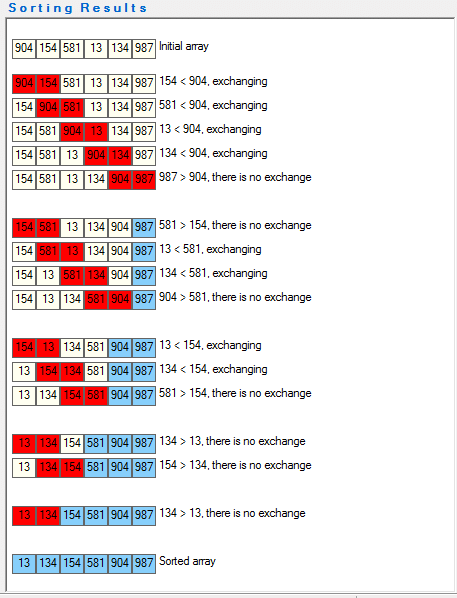
\includegraphics[scale=0.5]{img/Obtained-result-using-Bubble-sort-algorithm-and-array-with-six-elements.png}
    \caption{Corrida de Bubble Sort para un arreglo no ordenado (imagen sacada de Google).}
\end{figure}

A continuación, el código para el algoritmo de la burbuja\marginfootnote{Pseudocódigo sacado del Cormen.}:

\begin{algoritmo}
    \caption{Bubble Sort}\label{alg:bubble}
    \KwData{$A$ arreglo no ordenado}
    \KwResult{$A$ arreglo ordenado}
    \For{$i \leftarrow 1$ \textup{hasta} $length[A]$}{
        \For{$j \leftarrow length[A]$ \textup{hasta} $i+1$}{
        \If{$A[j] < A[j-1]$}{
        intercambia $A[j] \rightleftarrows A[j-1]$
        }
        }
    }
\end{algoritmo}

\break

Analicemos el algoritmo. Las operaciones son comparaciones e intercambio de valores. Así que, si el conjunto tiene $n$ elementos y esa es la medida de la instancia:

\begin{itemize}
    \item Para cada $j$ se hacen $n - j - 1$ comparaciones.
    \item Son $(n-1) + (n-2) + \dots + 2 + 1 = \frac{1}{2}n(n-1)$.
    \item Esto es $O(n^2)$.
    \item La cantidad de intercambios es también $O(n^2)$ (esto en el peor de los casos, se hace un intercambio después de cada comparación).
\end{itemize}

\textbf{En conclusión:} El algoritmo de la burbuja tiene eficiencia $O(n^2)$ en función de la cantidad de elementos del conjunto a ordenar.

Comparemos el algoritmo de la burbuja con una versión del algoritmo de inserción. El \textbf{algoritmo de inserción} construye una lista comenzando con el primer elemento del conjunto dado. Luego agrega el segundo elemento a la lista \textit{en el lugar correcto}. Y así sigue con los demás elementos del conjunto de manera que cada lista queda ordenada de una vez. La eficiencia de este algoritmo depende del método que se utilice para insertar el elemento \textit{en el lugar correcto}.

En nuestro caso, usaremos el método de \textbf{bisección}: Para insertar el $i$-ésimo elemento, se decide en cuál mitad de la lista debería ir. Después, en cuál mitad de esa mitad debería ir y así sucesivamente.

Ahora, analicemos este algoritmo:

\begin{itemize}
    \item Supongamos que el conjunto a ordenar tiene $n$ elementos.
    \item Si $n$ está entre $2^{r-1}$ y $2^r$, entonces hay que hacer $r$ comparaciones.
    \item En total son $\log_22 + \log_23 + \dots + \log_2 n$ comparaciones (aprox.).
    \item Esto es $O(n\log n)$.
\end{itemize}

\textbf{En conclusión}: El algoritmo de inserción, usando el método de bisección tiene eficiencia $O(n \log n)$. Pero al hacer la inserción en el lugar correcto, en el peor de los casos hay que intercambiar los términos de la lista. Esto serían otra vez $n^2$ intercambios. Por tanto, este algoritmo tiene también eficiencia $O(n^2)$.

\end{document}